
\subsection{Distributions}\label{distributions}

Let's imagine we will measure how long it takes to get from Brooklyn
College to Times square. Google maps says this takes about 54 minutes.
But, we all know that is an estimate that sometimes be off. Any given
trip could be shorter or longer. As a result, if we measured how long
several trips take for different people, we will find different times.
So, the population of travel times has variability. We can easily
describe these travel times with distributions. For example, consider
the two distributions below.

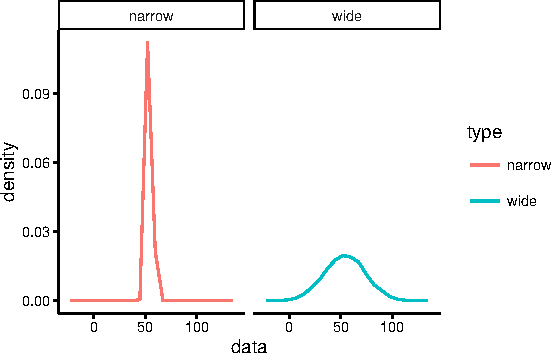
\includegraphics{Ttest_files/figure-latex/unnamed-chunk-1-1}

Both distributions have peaks around 54 minutes, which is the average
travel time between Brooklyn College and Times Square by subway. And,
both distributions have some variability. Some travel times are shorter
and some are longer than 54 minutes. The narrow distribution has less
variability than the wide distribution. For example, the narrow
distribution has a standard deviation of 2 minutes, and the wide
distribution has a standard deviation of 20 minutes.

What does the variability mean for your travel time? If there is less
variability, then more of your trips will be close to the mean of 54
minutes. And, when the trip is shorter or longer than 54 minutes, it
won't be too much shorter or longer, only a few minutes give or take.
Notice, that certain travel times pretty much never happen in the narrow
distribution. For example, it never takes 20 or a 100 minutes. When
there is more variability, then more of your trips will be slower or
faster than 54 minutes. For example, although the trips will average out
to 54 minutes, many trips will be much shorter, and much longer than 54
minutes. For example, you could expect a trip of 75 minutes to happen
fairly often. But, even when the distribution is wide, some very short
or long trips still do not happen very often. For example, a trip of 300
minutes never happens according to the wide distribution.

Randomly sampling a number from a distribution is a lot like taking your
chances on the subway. You might get to your destination in the average
time, or you could have bad luck and get on the train when there are a
lot of delays. We have a feeling for what the subway can do, it can
sometimes be fast and sometimes be slow. Similarly, by looking at a
distribution, we can get a feeling for what chance can do to the
measurement.

Whenever we take a measurement, we can think of it as taking a random
sample from a distribution. The distribution shows us that there are
different probabilities of getting smaller or larger numbers. The mean
is the most probable number, and in the distributions we are looking at,
as the numbers get smaller or larger, they also get less and less
likely. So, just by looking at the distribution, we can get a feeling
for what chance can do. For example, random sampling from the narrow
distribution will usually give numbers around 54, plus or minus 2 or
4ish. And, random sampling from the wide disribution will usually give
us numbers around 54, plus or minus 20-40ish.

\subsection{Differences can arise by chance because of
sampling}\label{differences-can-arise-by-chance-because-of-sampling}

Let's say you and your friend each take 10 subway trips between Brooklyn
College and Times Square, and each time you use your cell phone to
record how long each trip takes. This is the same as taking two samples
of 10 scores from the travel time distribution. What happens we we do
this? Will you and your friend have identical scores? Probably not. Each
time, different random factors will cause each of the trips to take
different amounts of time. We can plot the outcome of these hypothetical
trips below in a histogram.

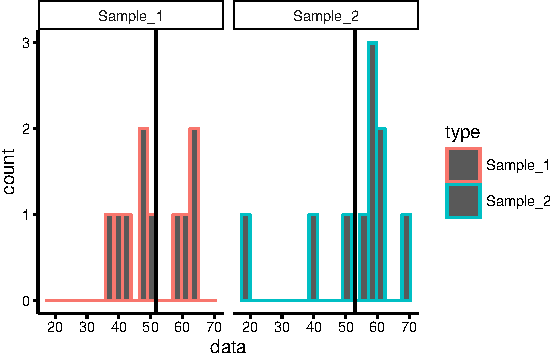
\includegraphics{Ttest_files/figure-latex/unnamed-chunk-2-1}

The histogram shows that in each sample, different trips took different
amounts of time. These samples were created by randomly picking numbers
from a normal distribution with mean = 54, and standard deviation = 20.
So, we might expect that both of our samples with also have a mean of
54. But, as you can see this is not true. The black lines on each of the
histograms show the mean travel times, and it is clear they are not
exactly the same.
\emph{The difference between these two sample means was produced by random chance.}

\subsection{What kind of differences can chance
produce?}\label{what-kind-of-differences-can-chance-produce}

Let's first look at the kind of differences that random sampling can
produce in our subway example. Imagine, that 20 people each took 10
trips between Brooklyn College and Times Square, and all of them
recorded their travel times. The data might look like this:

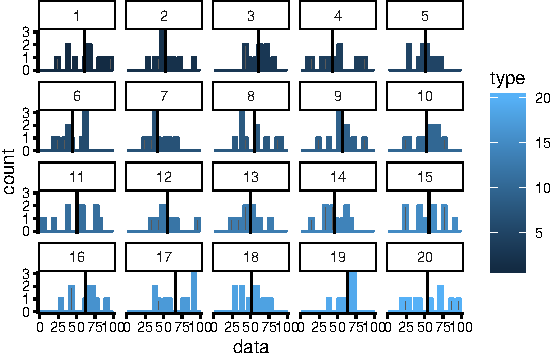
\includegraphics{Ttest_files/figure-latex/unnamed-chunk-3-1}

It easy to see that each person had different sets of travel times, and
that the means (black bars) are also moving around. All of the means are
close-ish to 54 minutes (which is the true mean), but some means are
smaller and larger. These sample means are very important, and they
point to another distribution, the sampling distribution of the mean.

The sampling distribution of the mean is a hypothetical idea. Imagine if
instead of 20 people taking 10 trips, and infinite number of people each
took 10 trips, and then recorded their travel times. Each of these
samples would have it's own mean. What does this distribution look like?
We can use a computer to simulate this distribution below:

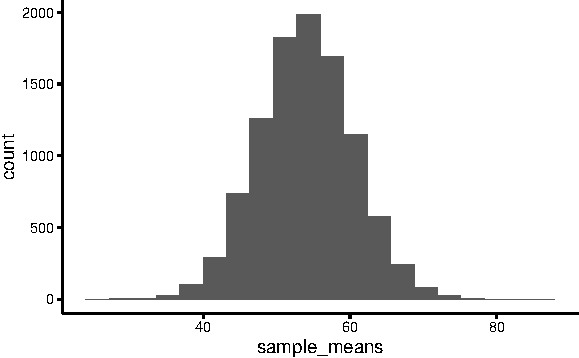
\includegraphics{Ttest_files/figure-latex/unnamed-chunk-4-1}

Remember each of the black lines in the sample histograms that represent
the sample means? The above histogram shows means from 10,000 of those
black lines (imagining we had 10,000 take trips).

We see that the distribution is centered on 54, which is the true mean
of the population. We also see that some means get as small as around
35, and as large as 75. However, sample means hardly ever get smaller
than 30, or larger than 80.

This graph is our window into the things that chance can do, and the
differences that random sampling can produce just by taking measurements
that have variability. What is most important, is that there are clearly
hard limits on what chance can do in this situation. We already said,
that chance alone hardly ever produces a mean larger than 75. We can use
this kind of information when we observe means that occur outside of our
chance window. For example, if one person had a sample mean of 5 minutes
for taking 10 trips, what can we infer? Well, we can say that chance has
an infintesimally small probability of producing this sample mean. For
this reason,we can also confidently rule-out chance as an explanation.
My guess is that person obviously DID NOT TAKE THE SUBWAY. Perhaps they
flew in a helicopter.

It easy to rule out chance when the measurement produces sample mean
that is well outside the chance window (like 5 minutes). It gets harder
to confidently rule out chance when the sample mean is inside the chance
window, but it can still be done. Researchers set their own criterions
about this issue (e.g., alpha value). For example, if you found a sample
mean of 70, what would you conclude? The histogram shows this sample
mean occurs with a very low frequency, which means it does occur by
chance. But, the chances are very low, less than 1\%. So, if you are
willing to accept those chances of being wrong, you might infer that a
sample mean of 75 was not produced by chance, but perhaps produced by
long delays on the subway.

\subsection{Chance can produce differences between conditions in an
experiment}\label{chance-can-produce-differences-between-conditions-in-an-experiment}

The reason we are spending so much time on understanding chance, is that
chance can produce differences between conditions in an experiment. This
occurs for the same reason that chance can produce different sample
means by random sampling alone. Remember in a simple experiment, we are
taking samples of the dependent variable in two conditions. We want to
know if there was a difference in the measure between conditions, so we
often look at the difference in sample means between the conditions.
And, as we have learned, those sample means can be different just
because of random chance.

Fortunately, we can use methods called inferential statistics to
estimate the kinds of differences that chance can produce. Then, we can
estimate the likelihood that the differences we observe were produced by
chance. When we find differences that are \emph{likely not} produced by
chance, we can be more confident that our observed differences are real,
and not random.

\section{2 level designs and t-tests}\label{level-designs-and-t-tests}

There are multiple ways to estimate whether chance is responsible for a
difference in an experiment. By far the most common approach is to use a
t-test. The t-test is a statitiscal method for analyzing the data in two
conditions to determine the likelihood that any observed difference
could have been produced by chance. You can refer to the inferential
statistics chapter, your old notes from statistics, discussions of
t-tests in the lab manual, and google t-tests to learn more about how
they work. For now, we will briefly describe the three different kinds
of t-tests, and give an example of how they are used to analyze data,
and how the results from a t-test are reported in journal article.

The three most common versions of the t-test are: one-sample t-test,
independent samples t-test, and the paired samples t-test. The one
sample t-test is used to test whether a sample mean could have come from
a particular population. The independent samples t-test is used in
between-subjects designs, to test whether the sample mean in one
condition is different from the sample mean in another condition. The
paired samples t-test is used in within-subjects designs, to test
whether the sample mean in one condition is different from the sample
mean in the other condition.

All t-tests give the same basic information, a t-value, and a p-value.
Simply, the p-value gives the probability that the observed difference
between means could have been produced by chance alone. If we dive into
the details, we will see that the p-value estimate depends on several
assumptions being met, and also has more nuanced meanings. But for now,
it gives us what we want, an estimate of the likelihood that chance
could have produced the difference we observed. When the p-value is very
small (e.g., less than .05, or 5\%), many researchers would conclude
that a difference ``statistically significant'', and probably not
produced by chance.

\subsection{An example}\label{an-example}

Imagine a between-subjects experiment on 20 student, asking whether
studying or not studying changes test performance on a midterm. The IV
is studying (Studying vs.~No-Studying), and the DV is test performance
(percentage on the midterm). Below are some imaginary results from the
experiment.

\begin{longtable}[]{@{}rr@{}}
\toprule
study & nostudy\tabularnewline
\midrule
\endhead
75 & 75\tabularnewline
82 & 79\tabularnewline
82 & 85\tabularnewline
86 & 75\tabularnewline
71 & 79\tabularnewline
78 & 73\tabularnewline
85 & 76\tabularnewline
77 & 75\tabularnewline
72 & 78\tabularnewline
74 & 67\tabularnewline
\bottomrule
\end{longtable}



